% Also that cellular skimmers are a thing http://newjersey.news12.com/story/38809657/consumer-alert-gas-station-gas-pump-credit-card-skimmers

% Also this is only going to get worse as the Bluetooth shimmer is now a thing https://www.sparkfun.com/sparkx/blog/2673

% "FICO, a credit scoring and analytics firm, noted that during the first half of 2017"

% https://www.muni.cz/en/research/publications/1073227
% https://www.muni.cz/en/research/publications/1362671
%
%European Financial Systems 2016, Proceedings of the 13th International Scientific Conference, year: 2016

%!TEX root = paper.tex
\section{Background}
\label{sec:background}

\begin{figure}
    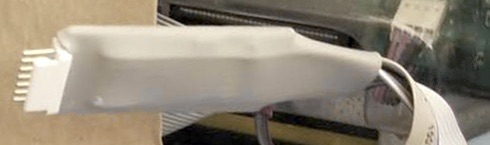
\includegraphics[width=0.95\linewidth]{skimmer/fig/wrapped-skimmer}
    \caption{An internal Bluetooth-based skimmer wrapped in grey tubing to blend in with the cabling inside the fuel pump. This skimmer
    was detected by \bluetana\ in Tempe, AZ.
%\noteby{NB}{Should we maybe put like a bigger picture with the entrails of the gas pump also visible?}}
}
\label{fig:wrapped-skimmer}
\end{figure}

\emph{Skimmers} are illicit devices that capture credit card magnetic stripe data when a card is used at a point-of-sale (PoS) terminal or automatic teller machine (ATM). External skimmers use a magnetic head concealed in a false
faceplate to read the magnetic stripe of a card as it is inserted into the real card reader. However, this paper is concerned
with a newer class of skimmers, called \emph{internal skimmers}, that are installed entirely inside a PoS
terminal or ATM, leaving no visual evidence of its presence~\cite{skimreaper2018}. Internal skimmers are attached inline to the cable that connects the
card reader to the main circuit board of the PoS terminal, tapping into the data and drawing power.
%
To make data collection easier, many internal skimmers include a Bluetooth-to-serial module that allows the
perpetrator to covertly collect the ``skimmed'' card data from a safe distance.
%
These skimmers are built using commodity hardware with a total unit cost of \$20 or less.

Fuel pumps
with a built-in PoS terminal have become a very popular target for such internal skimmers: they are unattended, easy
to access, and have poor physical security, which make it easy to install a skimmer without being noticed.
%
In a typical installation scenario, an attacker positions a van at a fuel station to block the station attendant's view of
the target pump (Excerpt in \ref{sec:appendix:cardsperskimmer}), opens the fuel pump using a common master key or crowbar, and clips a discreet gumstick-sized skimmer to the
ribbon cable between reader and main circuit board using a vampire clip (Figure~\ref{fig:wrapped-skimmer}). 
The entire process to install skimmer can
take less than 10 seconds~\cite{arizonareport}. The perpetrator can then return to the station with a 
smartphone, and without leaving their vehicle, connect to the skimmer using Bluetooth and download the card data.

\begin{figure}
    \centering
    \includegraphics[width=0.95\linewidth]{skimmer/fig/skimmer-example}
    \caption{Parts of a typical internal Bluetooth-based fuel pump skimmer. This skimmer
    was detected by \bluetana.}
    \label{fig:skimmer-example}
\end{figure}

\subsection{Internal Bluetooth Skimmers}
\label{sec:bkgd-skimhw}

The subject of our study are \emph{internal, Bluetooth-based skimmers} that are installed in fuel pump PoS
terminals. 
%
Figure~\ref{fig:skimmer-example} shows a typical Bluetooth skimmer, recovered from a fuel station in Southern California. This skimmer consists of a ``Teensy'' development board with an ARM Cortex-M4F
micro-controller and a Roving Networks \xspace{RN-42} Bluetooth-to-serial module. It also includes connectors 
for tapping into the wiring inside the pump (not shown). 

\paragraph{Connections} In the figure, the ribbon cable on the left intercepts or replaces the ribbon cable that connects the
magnetic stripe reader to the PoS terminal main board. The skimmer also uses this connection for power: the power and
ground pins of the Teensy (on far left of board, not visible in Figure~\ref{fig:skimmer-example}) are connected to
power and ground on the card reader cable. The ribbon cable on the right intercepts or replaces the ribbon cable from
the PoS keypad. This allows the perpetrator to capture additional card verification data, namely the debit card PIN
or credit card billing ZIP Code. Availability of a PIN code with a stolen debit card in particular, can increase its
value five-fold on the black market (Table \ref{tab:cardval}). However, not all skimmers capture keypad data.

Most gas station skimmers read the unencrypted data pulled from magnetic stripe readers.
%
Card issuers feel that removing sensitive data from the magnetic stripe on cards will help to solve
the problem~\cite{pcidss}.
%
Newer literature has demonstrated attacks on chip payment systems~\cite{bar2005known, bond2014chip}, and
law enforcement in Latin America have begun to find EMV skimmers that are Bluetooth enabled~\cite{krebshimmer,
customshimmer}.

\paragraph{Controller board} The skimmer pictured in Figure~\ref{fig:skimmer-example} used a Teensy micro-controller
development board equipped with a 120 MHz ARM Cortex-M4F micro-controller made by Freescale Semiconductor. By using a
development board, a skimmer requires only rudimentary electronic assembly: soldering wires to the development board.

However, skimmers have also been found using what appeared to be fully custom-designed boards. These are compact,
making them better for hiding in the dispenser. Examples of micro-controllers used in recovered skimmers include
Microchip PIC18F4550~\cite{sparkfunapp} and Atmel XMEGA128A4U~\cite{customshimmer}.

%\notefor{Nishant}{Please add additional examples of custom PCB skimmers from Web or skimmers we have seen ourselves; list \emph{exact} micro-controller and include a reference.}

%\noteby{NB}{Skimmers require minimal features on the micro-controller- low memory footprint[NB - Quote sparkfun website], two serial peripherals (to Bluetooth radio and mag reader), and a couple of GPIO/ADC(keypad) are all that are needed. In practice, skimmers recovered in the wild have been known to use various types of micro-controller boards.The first kind use readily available development boards, to enable fast prototyping. For example, the skimmer shown in figure uses a Teensy. In another kind of skimmers, criminals tend to simply re-purpose the micro-controller board on portable USB/Bluetooth mag readers, to use them as skimmers. The existing firmware can be used as is, but now to skim data. Finally, there are skimmers using custom boards based on a variety of micro-controllers (PIC18F, AtMega and others). While these boards take more effort to design and manufacture, the result is a compact skimmer which typically is hard to spot.}


\paragraph{Storage} The Teensy board also has a microSD card slot for additional data storage. Skimmers built on custom PCBs have also used flash and EEPROM ICs for storage. The storage capacities vary across designs, with examples using the PCT25VF032B (32-Mbit)~\cite{customshimmer} and M25P16VP (16-Mbit)~\cite{sparkfunapp}.

\paragraph{Bluetooth module} The skimmer shown in Figure~\ref{fig:skimmer-example} uses a Roving Networks RN-42 module, an inexpensive Bluetooth-to-serial module found in many skimmers. In Section~\ref{sec:bluetana:tool} we describe characteristics of popular Bluetooth-to-serial modules used in recovered skimmers for wireless data exfiltration. On the Bluetooth side, a Bluetooth-to-serial module provides a Serial Port Peripheral interface, which most operating systems recognize as a Bluetooth modem and instantiate a serial device for it. Operating systems will create a corresponding serial device, allowing user-space applications, namely a criminal's card dumping application, to communicate with the module. On the hardware side, a Bluetooth-to-serial module provides a TTL-level receive and transmit pin, allowing it to interface to any micro-controller UART. The module this allows even the simplest micro-controller to communicate via Bluetooth with a host device. The 2.4GHz Bluetooth antenna is included on the module's circuit board (exposed area to the left of the metal shield for the module shown in Figure~\ref{fig:skimmer-example}), so the antenna is also hidden.

Bluetooth-to-serial modules generally require no configuration, however, most
can be reconfigured using Hayes-style modem AT commands. In
Section~\ref{sec:bluetooth:skimmers} we describe the configuration capabilities
of popular modules. Notably, all of the Bluetooth-to-serial modules we found in
skimmers support changing the device MAC address, Bluetooth device name,
changing the pairing password, and the ability to become non-discoverable once
paired.

\subsection{Economics of Carding}
\label{sec:background:money}
Stealing and monetizing stolen credit and debit card data, called \emph{carding} by its practitioners, is a well-studied
form of financial fraud, however, reliable estimates of losses resulting from a single skimmer are difficult to find. To the criminal operating a skimmer, the expected revenue per skimmer breaks down as:
%
\[W = \textrm{(card value)}
\times \textrm{(cards per day)}
\times \textrm{(days deployed)}.\]
%\[W = \underbrace{\textrm{(card value)}}_{P}
%\times \underbrace{\textrm{(cards per day)}}_{Q}
%\times \underbrace{\textrm{(days deployed)}}_{D}.\]

Of these, we found published estimates for only the first two quantities, and very little about skimmer lifetimes. Here, we summarize the available data with the goal of estimating the losses incurred by a single skimmer.

\paragraph{Card value} To monetize stolen credit card data, skimmer installers have two options: sell the data on the black market, or cash out the cards on themselves. Based on our survey of sites selling stolen card data, black market prices for stolen cards fall in the \$10--220 range, depending on whether the card is a debit or credit card, and whether it comes with a PIN (for debit) or billing ZIP code (for credit). Table~\ref{tab:cardval} provides a summary of these prices with references. 

\begin{table}
\caption{Value of stolen credit and debit cards.}
\begin{tabular}{l@{\quad}lrl}
    \toprule
    \multicolumn{2}{l}{\colname{Scheme}} & \colname{Value} & \colname{Reference} \\
    \midrule
    \multicolumn{2}{l}{\textbf{Black market price}} \\
    & Debit, no PIN & \$20--30 & \cite{meccadumps,sellcvv,dumpsto, dumpsPrtShip} \\
    & Debit with PIN & \$110--220 & \cite{legitshop, sellcvv, dumpsPrtShip} \\
    & Credit, no ZIP & \$10--25 & \cite{meccadumps,sellcvv,dumpsto, dumpsPrtShip} \\
    & Credit with ZIP & \$25--60 & \cite{meccadumps,sellcvv,dumpsto, dumpsPrtShip} \\
    \multicolumn{2}{l}{\textbf{Cash-out value}} \\
    & Credit or Debit (standard) & \$400--800 & \cite{makingFirstMoney, cardingNewbieGuide, howToSucceedInStore, viceInterviewWithCarder} \\
    & Credit (premium) & \$1,000 & \cite{cardingNewbieGuide, santandWithdraw, honeyMoneyTut}\\
   \multicolumn{2}{l}{\textbf{Bank and merchant loss}} \\
%   & DOJ & \$902 & \cite{harrell2017} \\
%   & Arizona W\&M & \$1,003 & \cite{arizonareport} \\
    & Credit & \$1,003 & \cite{arizonareport} \\
%   & ATM Skimming & \$650 & \cite{ATMIA} \\
    & Debit & \$650 & \cite{ATMIA} \\
    \multicolumn{2}{l}{\textbf{Consumer liability}} \\
    & Debit (> 60 days) & unlimited & 15~USC~1693g \\ % \cite[\S1693g]{15uscode} \\
    & Debit (< 60 days) & max \$500 & 15~USC~1693g \\ % \cite[\S1693g]{15uscode} \\
    & Debit (< 2 days) & max \$50 & 15~USC~1693g \\ % \cite[\S1693g]{15uscode} \\
    & Credit & max \$50 & 15~USC~1643 \\ % \cite[\S1643]{15uscode} \\
     \multicolumn{2}{l}{\textbf{Prosecuted loss}} \\
%   & USSC & \$500 & \cite{ussc-guidelines} \\
    & Credit or debit & \$500 & \cite{ussc-guidelines} \\
     \multicolumn{2}{l}{\textbf{Court documents}} \\
     & Credit & \$362--400 & \cite{hristov,cristea,alisuretove,mekhakian} \\
     & Debit & \$665--1132 & \cite{estrada,aqel} \\

    \bottomrule
\end{tabular}

\label{tab:cardval}
\end{table}

Criminals can also cash out the cards themselves. Debit cards with a PIN are often cashed out by withdrawing money from an ATM, while credit cards are often cashed out by purchasing high-value merchandise (e.g. iPhones) and re-selling them. Reported cash-out values for debit and credit cards range between \$400 and \$1,000, depending on credit limit associated with the card.
%
We also conducted a survey of cash-out values reported in court documents involving skimmers.\footnote{We surveyed only documents available without fee from Court Listener.} Several cases reported specific cash-out values, rather than ranges. The debit card cash-out values were \$1132~\cite{hristov}, \$444~\cite{cristea} \$665~\cite{alisuretove}, \$1354~\cite{mekhakian}. The credit card cash-out values were \$362~\cite{aqel} and \$400~\cite{estrada}.

Losses due to credit and debit card fraud are borne largely by banks and merchants. This is likely because consumer liability for fraud in the U.S. is limited to \$50 for credit cards, and \$50 or more for debit cards (depending on how quickly the consumer reports the fraud).  Industry estimates for losses per-card incurred by banks are \$650 for debit cards and, \$1,003 for credit cards~\cite{arizonareport,ATMIA}. The U.S. Sentencing Commission estimates per-card losses at \$500 or more.

\paragraph{Cards per day} The number of cards a skimmer captures each day
depends on the number of transactions at that pump, which will vary by station.
Rippleshot, a payment fraud prevention service, states: ``a single compromised
pump can capture data from roughly 30--100 cards per day''~\cite{rippleshot}.
The lower end Rippleshot's estimate agrees with the estimate of 20--50 cards
per day we received from U.S. law enforcement agents. In addition, we found two
court documents that report criminals captured 25~\cite{estrada} and
30~\cite{alisuretove} cards per day.
%
We also studied 10 skimmers recovered from the field, which we were told were used and wiped daily. We found an average of 20 cards per skimmer, divided
evenly between debit and credit cards.\footnote{These skimmers were provided to
us because they were removed by the station owner, rather than LE, making them
unsuitable for use as evidence.}

\paragraph{Days deployed}  Internal skimmers are not limited by battery life
and can remain in operational indefinitely, because they draw power from the
PoS circuitry, Skimmer lifetime, then, is limited only by how long they can
remain undetected. Unfortunately, there is little reliable data on this. Our
only direct experience is our discovery of a pair of skimmers that remained
undetected for six months (Section~\ref{sec:blu:identify}). However, LE
informed us that criminals may leave skimmers in gas pumps after only a few days of retrieving 
card data and moving on to another location. Given the very limited data available on
skimmer lifetimes, we instead consider skimmer value \emph{per day of
operation}.

\paragraph{Cashout success rate}

Our analysis of court documents revealed that criminals are often unsuccessful
when trying to cashout a skimmed card. This may be due to a variety of reasons,
such as the following: incorrectly reading card data, hitting daily withdrawal
limits, and activating fraud alerts. Several cases mentioned that criminals
were not successful in cashing all skimmed cards. One case mentions a specific
cashout success rate of 47\%~\cite{mekhakian}.%, and the other was 50\%~\cite{rodriguez}.

\paragraph{Total skimmer value}

Finally, we estimate the range of per-day revenue from a skimmer based on the
prior figures. Our low end estimate is \$4,253 (25 cards per day, cashout of
\$362 per card, and 47\% cashout success rate), and our high end estimate is
\$63,638 (100 cards per day per day, \$1,354 cashout per card, and cashout success rate of
47\%).

\begin{comment}
Taking 30 cards per day, the lowest value in the Rippleshot range and near the middle of the estimate from law enforcement, and \$500 per card, the figure estimated by law enforcement officers and consistent with other estimates of cash-out value, places the value of each skimmer to the criminal at \textbf{\$15,000 per day}.

We compare this with a separate estimate obtained from information in court documents. Knowing that there is an equal distribution of credit and debit cards per skimmers, the average cashout value is at \$615 per card. With an average of 27 skimmer per card per day, and a lower bound success rate of 47.1\% in cashing out, the value of skimmer per day to the criminal stands at \$7820 per day.
\end{comment}

\begin{table}
\centering
\small
% Converted to vertical format by Aaron to manage space
\if 0
\begin{tabular}{lrrrrrrrrr}
\toprule
& \multicolumn{1}{c}{SD}
& \multicolumn{4}{c}{Arizona}
& \multicolumn{4}{c}{Florida}
\\
\cmidrule(lr){2-2}
\cmidrule(lr){3-6}
\cmidrule(lr){7-10}
%
\colname{Parameter}
& \colname{FY18}
& \colname{2016} & \colname{2017} & \colname{2018} & \colname{All}
& \colname{2016} & \colname{2017} & \colname{2018} & \colname{All}
\\
\midrule
Recovered skimmers
& \sdfyXVIIIskimmers
& \azXVIskimmers & \azXVIIskimmers & \azXVIIIskimmers & \azALLskimmers
& \flXVIskimmers & \flXVIIskimmers & \flXVIIIskimmers & \flALLskimmers
\\
Skimmed stations
& \sdfyXVIIIsksta
& \azXVIsksta & \azXVIIsksta & \azXVIIIsksta & \azALLsksta
& \flXVIsksta & \flXVIIsksta & \flXVIIIsksta & \flALLsksta
\\
Skimmers per incident
& \sdfyXVIIIskperinc
& \azXVIskperinc & \azXVIIskperinc & \azXVIIIskperinc & \azALLskperinc
& \flXVIskperinc & \flXVIIskperinc & \flXVIIIskperinc & \flALLskperinc
\\
Skimmers per million
& \sdfyXVIIIskpercap
& \azXVIskpercap & \azXVIIskpercap & \azXVIIIskpercap & \azALLskpercap
& \flXVIskpercap & \flXVIIskpercap & \flXVIIIskpercap & \flALLskpercap
\\
\bottomrule
\end{tabular}
\fi

\begin{tabular}{lcccc}
  \toprule
	\multicolumn{1}{p{1.5cm}}{\colname{Location \& Year}}          &
	\multicolumn{1}{p{2.0cm}}{\centering \colname{Recovered skimmers}}     & 
	\multicolumn{1}{p{1.5cm}}{\centering \colname{Skimmed stations}}       & 
	\multicolumn{1}{p{1.6cm}}{\centering \colname{Skimmers / \newline station}}     &
	\multicolumn{1}{p{1.8cm}}{\centering \colname{Skimmers / \newline $10^6$ people}}   \\
	\midrule
	\multicolumn{4}{l}{\textbf{San Diego}} & \\
	\hspace{0.4cm}FY 2018 & \sdfyXVIIIskimmers & \sdfyXVIIIsksta & \sdfyXVIIIskperinc & \sdfyXVIIIskpercap \\

  \multicolumn{4}{l}{\textbf{Arizona}} \\
	\hspace{0.4cm}2016 & \azXVIskimmers & \azXVIsksta & \azXVIskperinc & \azXVIskpercap \\
	\hspace{0.4cm}2017 & \azXVIIskimmers & \azXVIIsksta & \azXVIIskperinc & \azXVIIskpercap \\
	\hspace{0.4cm}2018 & \azXVIIIskimmers & \azXVIIIsksta & \azXVIIIskperinc & \azXVIIIskpercap \\
	\hspace{0.4cm}\textit{All}  & \azALLskimmers & \azALLsksta & \azALLskperinc & \azALLskpercap \\

  \multicolumn{4}{l}{\textbf{Florida}} \\
  \hspace{0.4cm}2016 & \flXVIskimmers & \flXVIsksta & \flXVIskperinc & \flXVIskpercap \\
	\hspace{0.4cm}2017 & \flXVIIskimmers & \flXVIIsksta & \flXVIIskperinc & \flXVIIskpercap \\
	\hspace{0.4cm}2018 & \flXVIIIskimmers & \flXVIIIsksta & \flXVIIIskperinc & \flXVIIIskpercap \\
	\hspace{0.4cm}\textit{All}  & \flALLskimmers & \flALLsksta & \flALLskperinc & \flALLskpercap \\

  \bottomrule
\end{tabular}

\caption{Prevalence of skimming in three regions of the U.S.}
\label{tab:wildskims}
\end{table}

\subsection{Skimmers Recovered in the Wild}
\label{sec:skimmersinwild}
To understand the prevalence of skimmers in the wild, we obtained data on recovered skimmers from three regions in the United States: San Diego and Imperial counties of California, with a combined population of 3.5 million; the state of Arizona, with a population of 7 million inhabitants; and the state of Florida, with a population of 21 million inhabitants. Table~\ref{tab:wildskims} summarizes the statistics. We note that these numbers do not represent \emph{all} recovered skimmers. For San Diego and Imperial counties, our statistics represent the number of skimmers found by or reported to a U.S. federal law enforcement agency. For Arizona and Florida, our statistics represent skimmers found by or reported to the AZWMSD and the Florida Department of Agriculture and Consumer Services.

The number of recovered skimmers has increased from 2016 to 2018 in both Florida and Arizona. The total number of skimmers recovered in 2018 across the three geographic regions is significant: if each skimmer operated for just one day, we estimate their total monetary impact would be ~\skimmerfraudXVIIIUSA. Yet, as the skimmers-per-million people number shows, the possibility of an average consumer encountering a skimmer at a gas station is quite small.
